
%Some information may be repeated from Lab4 as we are unsure on 100% of its contents
\section{Objectives}
By the end of this laboratory assignment, students are expected to learn how to 

\begin{itemize}

\item interface a DC motor with an embedded computer,
  
\item vary the rotational speed of a DC motor using pulse width modulation (PWM) signal, and 
  
\item measure the rotational speed of a DC motor using onboard quadrature encoder.  
 
  
\end{itemize}

\section{Parts}
\label{sec:partsDC_MotorBBBlue}
The main parts needed to conduct this laboratory experiment are: %
%
\begin{inparaenum}[a)]
% \item Breadboard,
\item BeagleBone Blue (BBBlue) embedded computer,
\item 2-cell lithium battery pack with connector,
\item One Micro-USB cable, 
\item Laptop computer, 
\item One 2-pin JST ZH connector,
\item One Pittmann DC motor,
\item One IN4004 Diode\footnote{\href{http://www.onsemi.com/pub/Collateral/1N4001-D.PDF}{http://www.onsemi.com/pub/Collateral/1N4001-D.PDF}},
\item Power supply,
\item Two 2N2222A transistors\footnote{\href{http://www.st.com/web/en/resource/technical/document/datasheet/CD00003223.pdf}{http://www.st.com/web/en/resource/technical/document/datasheet/CD00003223.pdf}},
\item Two $10~[\si{\kilo\ohm}]$ resistors,
\item Two $100~[\si{\kilo\ohm}]$ resistors,
\item Two $1~[\si{\kilo\ohm}]$ resistors, and 
\item Oscilloscope.  
% \item Function generator.
\end{inparaenum}


\section{Software}
\begin{enumerate}
    \item WinSCP
    \item PuTTY
\end{enumerate}



\section{Introduction}
\label{sec:introductionDC-MotorModeling}
Controlling of DC motor speed is of paramount importance due to its wide range of applications, such as fans, blowers, cranes, among others. The main purpose of this laboratory assignment is to vary the speed of a DC motor using an embedded computer, BBBlue. Therefore, this laboratory is divided into two separate parts. In this first part, an embedded computer will drive a DC motor at a certain speed. In the second part, the speed of the DC motor will be measured using electro-mechanical device called quadrature encoder. In the following, a brief illustration of these two parts is provided. 

\subsection{Driving DC Motor}

Figure~\ref{fig:dcMotorBBBlueBD} shows the block diagram for driving a DC motor shaft using a  BeagleBone Blue (BBBlue) embedded computer. The embedded computer outputs a analog voltage $V_s$ which is then mapped to the applied voltage $V_a$ range through an output signal conditioning circuit.  
%
\begin{figure}
  \centering
  \fcolorbox{white}{gray!20}{
              \begin{tikzpicture}
                % \tikzstyle{every node} = [font =\tiny]
                % \tikzstyle{block} = [draw, fill=blue!20, rectangle, 
                % minimum height=3em, minimum width=6em]
                \tikzstyle{block} = [draw, fill=blue!20, rectangle, rounded corners]      
                \tikzstyle{pinstyle} = [pin edge={to-,thin,black}]
                \node [block,text width=2.5cm,text centered] (BBBlue) {BBBlue embedded computer};
                \node[block, text width=2.5cm, text centered, right of =BBBlue, node distance=3.5cm](outSignalConditioning){Output signal conditioning};
                \node[block, text width=2.0cm, text centered, right of =outSignalConditioning, node distance=3.5cm](dcMotor){DC motor with shaft};                
                % Draw arrows
                \draw[->] (BBBlue) -- node[midway,above]{$V_s$}  (outSignalConditioning);
                \draw[->] (outSignalConditioning) -- node[midway,above]{$V_a$}  (dcMotor);
                \draw[->](dcMotor) -- ++(3*\smgrid,0)node[right]{Shaft speed};
              \end{tikzpicture}
  }            
  \caption{Block diagram of driving a DC motor using BBBlue embedded computer.}
  \label{fig:dcMotorBBBlueBD}
\end{figure}
%
The output signal conditioning circuit can be implemented using inverting amplifiers as shown in Figure~\ref{fig:outputSignalConditioning}. 
%
\begin{figure}
  \centering
  \begin{circuitikz}[scale=1,american voltages]
    \draw
    (0,0) node[op amp,fill=cyan!50] (opamp1){}
    (-8*\smgrid,\smgrid) node[left]{$V_s$} to[R,l^=$R_1$,o-*](opamp1.-)
    (opamp1.+)to[short,-*](opamp1.+)node[ground]{};
    \node at(0,0){\#1};
    \draw
    (opamp1.-) to[short,-](-2.4*\smgrid,4*\smgrid) to[R,l^=$R_f$](2.4*\smgrid,4*\smgrid) to[short,-*](opamp1.out);
    
    \draw
    (10*\smgrid,-\smgrid) node[op amp,fill=cyan!50](opamp2){}
    (opamp1.out) to[R,l^=$R$,-*](opamp2.-)
    (opamp2.-) to[short,-](7.5*\smgrid,4*\smgrid) to[R,l^=$R$](12.4*\smgrid,4*\smgrid) to[short,-*](opamp2.out);
    \node at(10*\smgrid,-\smgrid){\#2};
    \draw 
    (opamp2.+) to[short,-*](opamp2.+)node[ground]{};
    
    \draw
    (opamp2.out) to[short,-o](14*\smgrid,-\smgrid) node[right]{$V_a$};
    
  \end{circuitikz}
  \caption{A possible output signal conditioning circuit using op-amps.}
  \label{fig:outputSignalConditioning}
\end{figure}
%
Note that the analog output voltage $V_s$ is generated by BBBlue using a PWM signal. A PWM signal is a form of a digitally encoded analog signal. There are two main components of a PWM signal: the duty cycle and the period. As with any other digital signal, a PWM signal is a mixture of high and low values (logic 1 and logic 0). The period, as with any other signal, is the time taken for a full cycle of the signal. The duty cycle, on the other hand, is the fraction of the time that the signal is high (logic value 1 or \emph{on time}) with respect to the signal period. It is expressed in percent as:
%
\begin{align*}
  \text{Duty cycle}(\%) = \frac{\text{On time}}{\text{Time period}}\times 100\%.
\end{align*}
%
By varying the \emph{duty cycle}, one can vary the rotational speed of a DC motor. The robotics cape hardware embedded in the BBBlue single-board computer has four DC motor channels. It can drive four DC motors bidirectionally powered only from a 2-cell lithium battery pack connected to the cape\footnote{\href{http://strawsondesign.com/docs/librobotcontrol/group___motor.html}{http://strawsondesign.com/docs/librobotcontrol/group\_\_\_motor.html}}. Note taht each channel supports up to $1.2~[\ampere]$ of current. Therefore, a careful consideration needs to be exercised when choosing DC motors which will not exceed this ranting of current. Each channel can be connected to the output signal conditioning circuit using a 2-pin JST ZH connector. To drive the DC motor using PWM signals provided by BBBlue, the \emph{librobotcontrol} library will be used. The following functions\footnote{Description of these functions are taken from http://www.strawsondesign.com/} from the \emph{librobotcontrol} library are useful when writing a program for the BBBlue that drives a DC motor. % 
%

\begin{tabular}{l|p{3.5in}}
    \toprule
     Function & Description\\
     \toprule
     int 	rc\_motor\_init (void) & Initializes all 4 motors and leaves them in a free-spin (0 throttle) state.\\
     \hline 
     int 	rc\_motor\_init\_freq (int pwm\_frequency\_hz) & Set the pwm frequency\\
     \hline 
    int 	rc\_motor\_set (int ch, double duty) & Sets the bidirectional duty cycle (power) to a single motor or all motors if $0$ is provided as a channel\\
     \hline 
    int 	rc\_motor\_cleanup (void) & Puts all $4$ motors into a free-spin ($0$ throttle) state, puts the h-bridges into standby mode, and closes all file pointers to GPIO and PWM systems\\
     \hline 
    int 	rc\_motor\_free\_spin (int ch) & Puts a motor into a zero-throttle state allowing it to spin freely\\
     \hline 
    int 	rc\_motor\_brake (int ch) & Connects the motor terminal pairs together which makes the motor fight against its own back EMF turning it into a brake resisting rotation\\    
     \bottomrule
\end{tabular}
%

\subsection{DC Motor Speed Measurement}
The general high-level block diagram to measure rotational speed of a DC motor is shown in Figure~\ref{fig:dcMotorBBBlueBD1}. It is assumed that a DC motor has a rotary encoder (quadrature encoder, for instance) mounted on it. The angular motion of the rotor of a DC motor is detected by its onboard rotary encoder which then produces analog or digital (pulse) signals. The input signal conditioning circuit generates digital signals that correspond to the analog motion of the DC motor. The digital signals are then fed to the embedded computer to compute the  corresponding rotational speed. 
%
\begin{figure}
  \centering
  \fcolorbox{white}{gray!20}{
              \begin{tikzpicture}
                % \tikzstyle{every node} = [font =\tiny]
                % \tikzstyle{block} = [draw, fill=blue!20, rectangle, 
                % minimum height=3em, minimum width=6em]
                \tikzstyle{block} = [draw, fill=blue!20, rectangle, rounded corners]      
                \tikzstyle{pinstyle} = [pin edge={to-,thin,black}]
                \node [block,text width=1.75cm, text centered] (dcMotor) {DC motor};
                \node[block, text width=2.6cm, text centered, right of =dcMotor, node distance=4.0cm](rotaryEncoder){Speed sensor (rotary encoder)};
                \node[block, text width=2.25cm, text centered, right of =rotaryEncoder, node distance=5.0cm](inSignalConditioning1){Input signal conditioning};                
                \node[block, text width=2.0cm, text centered, right of =inSignalConditioning1, node distance=3.5cm](BBBlue){Embedded computer};                                
                % Draw arrows
                \draw[->] (dcMotor) -- node[midway,above]{Angular }  (rotaryEncoder);
                \draw[->] (dcMotor) -- node[midway,below]{motion}  (rotaryEncoder);                
                \draw[->] (rotaryEncoder) -- node[midway,above]{Square wave}  (inSignalConditioning1);
                \draw[->] (rotaryEncoder) -- node[midway,below]{(pulse)}  (inSignalConditioning1);
                \draw[->] (inSignalConditioning1) -- node[midway,above]{Digital}  (BBBlue);
                \draw[->] (inSignalConditioning1) -- node[midway,below]{signal}  (BBBlue);                
                \draw[->](BBBlue) -- ++(3*\smgrid,0)node[above right]{Shaft speed};
                \draw[->](BBBlue) -- ++(3*\smgrid,0)node[below right]{(computed)};                
              \end{tikzpicture}
}              
  \caption{Block diagram of measuring a DC motor speed using BBBlue embedded computer.}
  \label{fig:dcMotorBBBlueBD1}
\end{figure}
%
Figure~\ref{fig:rotaryEncoderInterface} shows a possible way to interface  a DC motor kit with an embedded computer (in this case, a BBBlue) in measuring shaft speed using an onboard quadrature encoder. %
%
\begin{figure}
  \centering
  \fcolorbox{white}{blue!15}{
    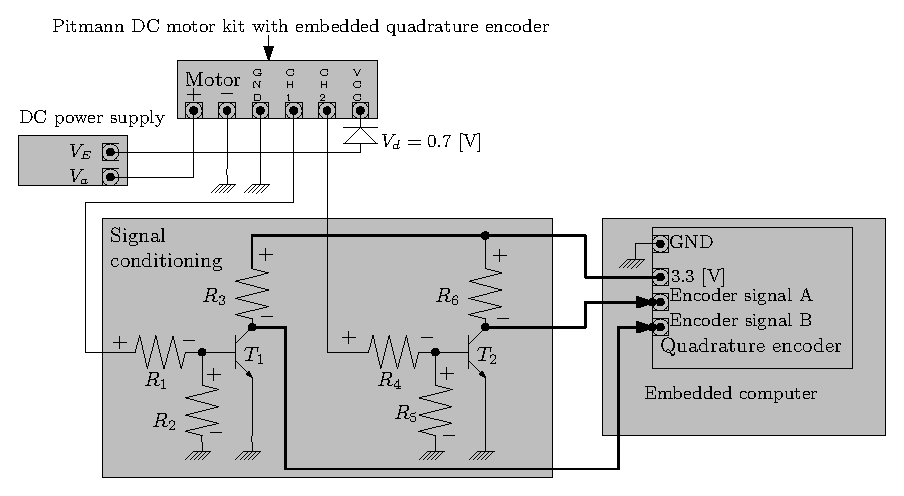
\includegraphics[width=0.6\textwidth]{figs/ipe/rotaryEncoderInterface}
    }
  \caption[DC motor interface circuit with embedded computer.]{Interface circuit for measuring rotational speed of a DC motor using an onboard quadrature encoder of an embedded computer.  }
  \label{fig:rotaryEncoderInterface}
\end{figure}
%
The DC motor in the Pittmann DC motor kit takes applied voltage from a DC power supply. The motor kit has an embedded rotary encoder (quadrature encoder) mounted on it. The encoder circuit in the motor kit is powered with a $5~[\volt]$ DC power supply. The diode is used to protect the encoder circuit connected with a power supply from reverse polarity. Quadrature encoder outputs square wave pulse with an amplitude of $~\approx 5~[\volt].$ However, the quadrature encoder onboard the embedded computer (in the case, the BBBlue) accepts signals of amplitudes up to  $3.3~[\volt].$ Therefore, a signal conditioning circuit is designed to reduce square wave pulse  (generated by the quadrature encoder of the DC motor kit) amplitude.  

\begin{prelab}[DC motor programming]
  ~

  \begin{enumerate}
  \item Draw a flowchart (not handwritten!)  of the algorithm for your BBBlue that varies the duty cycle of a PWM signal.
    
  \item Draw a flowchart (not handwritten!)  of the algorithm for your BBBlue that reads digital signals entered into the onboard quadrature encoder  of the BBBlue and computes the motor shaft speed (in RPM) from channel $\#1$ or channel $\#2.$ 
  \end{enumerate}
\end{prelab}

\section{Laboratory Work}
The laboratory work consists of two parts. In the first part, the BBBlue embedded computer will be used to drive a DC motor for various applied voltages. In the second part, the shaft speed of a Pittmann DC motor  will be measured using an onboard quadrature encoder of the BBBlue embedded computer.

\subsection{Part 1 - Driving DC motor with PWM signal}

\begin{enumerate}

  
\item Connect a $2$-pin JST ZH connector with the DC motor driver channel $\#1.$
  
\item Design and construct the output signal conditioning circuit shown in the block diagram of Figure~\ref{fig:dcMotorBBBlueBD}.

\item Connect a 2-cell lithium battery pack (make sure to check for enough charge in the battery) to the robotics cape embedded into the BBBlue computer.     

% \begin{mdframed}
%   \textbf{BEFORE TESTING THE FULL CIRCUIT! Use the oscilloscope at your workstation to check the PWM signal generated from a function generator before applying that signal from your BeagleBone Blue.}
% \end{mdframed}

%have them test the circuit with the function generator and oscilloscope before attempting to use the BBB and encoder.
  
\item Write a program for your BBBlue that varies the duty cycle of a PWM signal. Measure the output voltages of the DC motor driver channel  and the output voltage of the output signal conditioning circuit. Then, complete the following table. ~\label{enum:dutyCycle}%
  
%
  \begin{center}
    \begin{tabular}{c|c|c}
      \toprule
      Duty cycle &  $V_s$ & $V_a$\\
      \toprule
      $100~\%$ & $\ldots$ & $\ldots$\\   %|| V_s =, V_a =
      $75~\%$ & $\ldots$ & $\ldots$\\   %|| V_s =, V_a =
      $50~\%$ & $\ldots$ & $\ldots$\\   %|| V_s =, V_a =
      $25~\%$ & $\ldots$ & $\ldots$\\   %|| V_s =, V_a =
      $0~\%$ & $\ldots$ & $\ldots$\\   %|| V_s =, V_a =      
      \bottomrule
    \end{tabular}    
  \end{center}
 
\item Use the Agilent E3630 $\mathbf{0}$-$\mathbf{6}~[\volt]$ option  as the voltage source $V_E$ to supply $V_E = 5.7~[\volt]$ to the rotary encoder of the motor.
\item Connect channel~$\#1$ (or channel~$\#2$) of the rotary encoder mounted on the DC motor's kit to channel~$\#1$ of the oscilloscope at your workstation.   
\item For $100\%$ duty cycle computed in Step~\ref{enum:dutyCycle}, apply the corresponding voltage $V_a$ to the \emph{Motor $\pm$ terminals} and record the speed by observing the pulse waveform on the oscilloscope. Note that the rotary encoder produces $500$ pulses per revolution. Repeat for $75\%,~50\%,~25\%,$ and $0\%$ duty cycle and record the measured motor speed in the table below: %
%
%
  \begin{center}
    \begin{tabular}{c|c|c|c|c|c}
      \toprule
      Duty cycle &  $V_s~[\volt]$ & $V_a~[\volt]$&$\omega_{0,\mathrm{shaft}}$ (measured) ~[RPM]&  $\omega_{0,\mathrm{shaft}}$ (computed) ~[RPM] & Error (\%)\\
      \toprule
      $100~\%$ & $\ldots$ & $\ldots$& $\ldots$ & $\ldots$ & $\ldots$\\   %|| V_s =, V_a =
      $75~\%$ & $\ldots$ & $\ldots$& $\ldots$ & $\ldots$ & $\ldots$\\   %|| V_s =, V_a =
      $50~\%$ & $\ldots$ & $\ldots$& $\ldots$ & $\ldots$ & $\ldots$\\   %|| V_s =, V_a =
      $25~\%$ & $\ldots$ & $\ldots$& $\ldots$ & $\ldots$ & $\ldots$\\   %|| V_s =, V_a =
      $0~\%$ & $\ldots$ & $\ldots$& $\ldots$ & $\ldots$ & $\ldots$\\   %|| V_s =, V_a =      
      \bottomrule
    \end{tabular}    
  \end{center}
  %
  
\end{enumerate}

\subsection{Part 2 - Measure DC motor shaft speed using quadrature encoder}

\begin{enumerate}
\item Measure the resistance of the $1~[\kilo\ohm],$ $10~[\kilo\ohm],$ $100~[\kilo\ohm]$  resistors $(R_1,R_2,R_3,R_4,R_5$ and $R_6).$ Then, complete the following table.

  \begin{center}
    \begin{tabular}{c|c|c}
      \toprule
      Quantity &  Ideal & Measured\\
      \toprule
      $R_1$ & $1~[\kilo\ohm]$ & $\ldots$\\   %|| R_1 =
      $R_2$ & $100~[\kilo\ohm]$ & $\ldots$\\   %|| R_2 =       
      $R_3$ & $10~[\kilo\ohm]$ & $\ldots$\\   %|| R_3 =
      $R_4$ & $1~[\kilo\ohm]$ & $\ldots$\\   %|| R_4 =
      $R_5$ & $100~[\kilo\ohm]$ & $\ldots$\\   %|| R_3 =
      $R_6$ & $1~[\kilo\ohm]$ & $\ldots$\\   %|| R_4 =             
      \bottomrule
    \end{tabular}    
  \end{center}
  
\item Construct the circuit shown in Figure~\ref{fig:rotaryEncoderInterface} using the components measured in the previous step.

 
\item Write a program for your BBBlue  that reads digital signals entered into the onboard quadrature encoder  of the BBBlue and computes the motor shaft speed from channel $\#1$ or channel $\#2.$ 
\item Use $30$V HP 6215  power supply to supply $V_a=4~[\volt]$ to the \emph{Motor $\pm$  terminals}  and record the speed computed by the program you wrote in the previous step. Repeat for $V_a=8~[\volt],~\ldots,~24~[\volt]$ and record the measured motor speed in the table below: %
%
  \begin{center}
    \begin{tabular}{c|c|c|c}
      \toprule
      $V_a~[\volt]$ &  $\omega_{0,\mathrm{shaft}}$ (measured) ~[rpm]&  $\omega_{0,\mathrm{shaft}}$ (computed) ~[rpm] & Error (\%)\\
      \toprule
      $0$ & $\ldots$ & $\ldots$& $\ldots$\\
      $4$ & $\ldots$ & $\ldots$& $\ldots$ \\
      $8$ & $\ldots$ & $\ldots$& $\ldots$ \\
      $12$ & $\ldots$ & $\ldots$& $\ldots$ \\
      $16$ & $\ldots$ & $\ldots$& $\ldots$ \\
      $20$ & $\ldots$ & $\ldots$& $\ldots$ \\
      $24$ & $\ldots$ & $\ldots$& $\ldots$ \\
      \bottomrule
    \end{tabular}    
  \end{center}

\item Connect the ammeter in series with the armature circuit of the motor as shown in Figure~\ref{fig:DC-MotorSchematicMeasuringNoLoadCurrent} and measure the no-load current for the motor's applied voltage $V_a=0,~4~[\volt],~8~[\volt],~\ldots,~24~[\volt].$ Record the measured no-load current in the table below: %
%
  \begin{center}
    \begin{tabular}{c|c|c|c}
      \toprule
      $V_a~[\volt]$ &  $I_0$ (measured) ~[\ampere]&  $I_0$ (computed) ~[\ampere] & Error (\%)\\
      \toprule
      $0$ & $\ldots$ & $\ldots$& $\ldots$\\
      $4$ & $\ldots$ & $\ldots$& $\ldots$ \\
      $8$ & $\ldots$ & $\ldots$& $\ldots$ \\
      $12$ & $\ldots$ & $\ldots$& $\ldots$ \\
      $16$ & $\ldots$ & $\ldots$& $\ldots$ \\
      $20$ & $\ldots$ & $\ldots$& $\ldots$ \\
      $24$ & $\ldots$ & $\ldots$& $\ldots$ \\
      \bottomrule
    \end{tabular}    
  \end{center}  



\item Comment on any discrepancy found between the computed and the experimental (measured) values of the no-load speeds  and and no-load currents. 

  
\end{enumerate}



%%% Local Variables:
%%% mode: latex
%%% TeX-master: "../../labBookMechatronics-V2"
%%% End:
